

\section{Experiments}
\label{sec:exp}

We conduct our experiments on PASCAL VOC 2007, PASCAL VOC 2012~\cite{voc} and MS COCO~\cite{coco} datasets. As is standard practice, we perform most of the ablative studies on the PASCAL VOC 2007 dataset. We also report our numbers on the PASCAL VOC 2012 and COCO dataset. Finally, we perform a comparison between our method and the Online Hard Example Mining (OHEM)~\cite{shrivastavaOHEM} approach. 




\begin{table*}[t]
\centering
\caption[caption]{\small {\bf VOC 2007 test} detection average precision (\%).  FRCN\raisebox{0.2ex}{$\star$} refers to FRCN \protect\cite{frcn} with our training schedule.}
\vspace{-0.1in}

\renewcommand{\arraystretch}{1.2}
\renewcommand{\tabcolsep}{1.2mm}
\resizebox{\linewidth}{!}{

\begin{tabular}{@{}L{2.1cm} !{\color{gray}\vrule}  L{1.2cm}   l r*{19}{x} @{}}
\Xhline{1pt}
method  & arch & mAP & aero      & bike      & bird      & boat      & bottle     & bus        & car        & cat        & chair      & cow        & table      & dog        & horse      & mbike      & persn     & plant      & sheep      & sofa       & train      & tv   \\
\Xhline{0.8pt}

FRCN~\cite{frcn}  &AlexNet  & 55.4 & 67.2 & 71.8 & 51.2 & 38.7 & 20.8 & 65.8 & 67.7 & 71.0 & 28.2 & 61.2 & 61.6 & 62.6 & 72.0 & 66.0 & 54.2 & 21.8 & 52.0 & 53.8 & 66.4 & 53.9 \\
FRCN\raisebox{0.2ex}{$\star$} &AlexNet  &57.0 & 67.3 & 72.1 & 54.0 & 38.3 & 24.4 & 65.7 & 70.7 & 66.9 & 32.4 & 60.2 & 63.2 & 62.5 & 72.4 & 67.6 & 59.2 & 24.1 & 53.0 & 60.6 & 64.0 & 61.5 \\
Ours (ASTN)  &AlexNet  & 58.1  & 68.7 & 73.4 & 53.9 & 36.9 & 26.5 & 69.4 & 71.8 & 68.7 & 33.0 & 60.6 & 64.0 & 60.9 & 76.5 & 70.6 & 60.9 & 25.2 & 55.2 & 56.9 & 68.3 & 59.9 \\
Ours (ASDN)  &AlexNet  & 58.5 & 67.1 & 72.0 & 53.4 & 36.4 & 25.3 & 68.5 & 71.8 & 70.0 & 34.7 & 63.1 & 64.5 & 64.3 & 75.5 & 70.0 & 61.5 & 26.8 & 55.3 & 58.2 & 70.5 & 60.5 \\
Ours (full)  &AlexNet  & 58.9 & 67.6 & 74.8 & 53.8 & 38.2 & 25.2 & 69.1 & 72.4 & 68.8 & 34.5 & 63.0 & 66.2 & 63.6 & 75.0 & 70.8 & 61.6 & 26.9 & 55.7 & 57.8 & 71.7 & 60.6 \\

\Xhline{0.5pt}
FRCN~\cite{frcn}  &VGG & 66.9 & 74.5 & 78.3 & 69.2 & 53.2 & 36.6 & 77.3 & 78.2 & 82.0 & 40.7 & 72.7 & 67.9 & 79.6 & 79.2 & 73.0 & 69.0 & 30.1 & 65.4 & 70.2 & 75.8 & 65.8 \\
%OHEM~\cite{shrivastavaOHEM}  &VGG  & {69.9} & 71.2 & 78.3 & 69.2 & 57.9 & 46.5 & 81.8 & 79.1 & 83.2 & 47.9 & 76.2 & 68.9 & 83.2 & 80.8 & 75.8 & 72.7 & 39.9 & 67.5 & 66.2 & 75.6 & 75.9 \\
FRCN\raisebox{0.2ex}{$\star$} &VGG  & 69.1 & 75.4 & 80.8 & 67.3 & 59.9 & 37.6 & 81.9 & 80.0 & 84.5 & 50.0 & 77.1 & 68.2 & 81.0 & 82.5 & 74.3 & 69.9 & 28.4 & 71.1 & 70.2 & 75.8 & 66.6  \\
Ours (ASTN)  &VGG  & 69.9 & 73.7 & 81.5 & 66.0 & 53.1 & 45.2 & 82.2 & 79.3 & 82.7 & 53.1 & 75.8 & 72.3 & 81.8 & 81.6 & 75.6 & 72.6 & 36.6 & 66.3 & 69.2 & 76.6 & 72.7  \\
Ours (ASDN)  &VGG  & 71.0 & 74.4 & 81.3 & 67.6 & 57.0 & 46.6 & 81.0 & 79.3 & 86.0 & 52.9 & 75.9 & 73.7 & 82.6 & 83.2 & 77.7 & 72.7 & 37.4 & 66.3 & 71.2 & 78.2 & 74.3 \\
Ours (full)  &VGG  & 71.4 & 75.7 & 83.6 & 68.4 & 58.0 & 44.7 & 81.9 & 80.4 & 86.3 & 53.7 & 76.1 & 72.5 & 82.6 & 83.9 & 77.1 & 73.1 & 38.1 & 70.0 & 69.7 & 78.8 & 73.1 \\

\Xhline{0.5pt}
FRCN\raisebox{0.2ex}{$\star$} &ResNet  & 71.8 & 78.7 & 82.2 & 71.8 & 55.1 & 41.7 & 79.5 & 80.8 & 88.5 & 53.4 & 81.8 & 72.1 & 87.6 & 85.2 & 80.0 & 72.0 & 35.5 & 71.6 & 75.8 & 78.3 & 64.3  \\
Ours (full)  &ResNet  & 73.6 &  75.4 & 83.8 & 75.1 & 61.3 & 44.8 & 81.9 & 81.1 & 87.9 & 57.9 & 81.2 & 72.5 & 87.6 & 85.2 & 80.3 & 74.7 & 44.3 & 72.2 & 76.7 & 76.9 & 71.4 \\

\Xhline{1pt}

\end{tabular}
}
\vspace{-0.05in}
\label{tab:voc2007}
\end{table*}




\begin{table*}[t]
\centering
\caption[caption]{\small {\bf VOC 2007 test} detection average precision (\%). Ablative analysis on the Adversarial Spatial Dropout Network.FRCN\raisebox{0.2ex}{$\star$} refers to FRCN \protect\cite{frcn} with our training schedule.}
\vspace{-0.1in}
%we can only report numbers from FRCN and mention FRCN* in text for 66.9 \vs 67.2.
%Options: Ours, OHEM [ours], FRCN+OHEM [ours]
\renewcommand{\arraystretch}{1.2}
\renewcommand{\tabcolsep}{1.2mm}
\resizebox{\linewidth}{!}{
%  \begin{tabular}{@{}L{2.4cm}|L{1.5cm}|r*{19}{x}|x@{}}
\begin{tabular}{@{}L{3.3cm} !{\color{gray}\vrule}  L{1.2cm}  !{\color{gray}\vrule}   l  !{\color{gray}\vrule}  r*{19}{x} @{}}
\Xhline{1pt}
method  & arch & mAP & aero      & bike      & bird      & boat      & bottle     & bus        & car        & cat        & chair      & cow        & table      & dog        & horse      & mbike      & persn     & plant      & sheep      & sofa       & train      & tv   \\
\Xhline{0.8pt}

FRCN\raisebox{0.2ex}{$\star$} &AlexNet  &57.0 & 67.3 & 72.1 & 54.0 & 38.3 & 24.4 & 65.7 & 70.7 & 66.9 & 32.4 & 60.2 & 63.2 & 62.5 & 72.4 & 67.6 & 59.2 & 24.1 & 53.0 & 60.6 & 64.0 & 61.5 \\
Ours (random dropout)  &AlexNet  & 57.3 & 68.6 & 72.6 & 52.0 & 34.7 & 26.9 & 64.1 & 71.3 & 67.1 & 33.8 & 60.3 & 62.0 & 62.7 & 73.5 & 70.4 & 59.8 & 25.7 & 53.0 & 58.8 & 68.6 & 60.9 \\
Ours (hard dropout)  &AlexNet  & 57.7  & 66.3 & 72.1 & 52.8 & 32.8 & 24.3 & 66.8 & 71.7 & 69.4 & 33.4 & 61.5 & 62.0 & 63.4 & 76.5 & 69.6 & 60.6 & 24.4 & 56.5 & 59.1 & 68.5 & 62.0 \\
Ours (fixed ASDN)  &AlexNet  & 57.5 & 66.3 & 72.7 & 50.4 & 36.6 & 24.5 & 66.4 & 71.1 & 68.8 & 34.7 & 61.2 & 64.1 & 61.9 & 74.4 & 69.4 & 60.4 & 26.8 & 55.1 & 57.2 & 68.6 & 60.1 \\
Ours (joint learning) &AlexNet & 58.5 & 67.1 & 72.0 & 53.4 & 36.4 & 25.3 & 68.5 & 71.8 & 70.0 & 34.7 & 63.1 & 64.5 & 64.3 & 75.5 & 70.0 & 61.5 & 26.8 & 55.3 & 58.2 & 70.5 & 60.5 \\

\Xhline{1pt}

\end{tabular}
}
\vspace{-0.05in}
\label{tab:voc2007_ab}
\end{table*}


\subsection{Experimental settings}

\textbf{PASCAL VOC.} For the VOC datasets, we use the `trainval' set for training and `test' set for testing.  We follow most of the setup in standard Fast-RCNN~\cite{frcn} for training. We apply SGD for 80K to train our models. The learning rate starts with $0.001$ and decreases to $0.0001$ after 60K iterations. We use the selective search proposals~\cite{Uijlings13} during training. 

\textbf{MS COCO.} For the COCO dataset, we use the `trainval35k' set for training and the  `minival' set for testing. During training the Fast-RCNN~\cite{frcn}, we apply SGD with 320K iterations. The learning rate starts with $0.001$ and decreases to $0.0001$ after 280K iterations. For object proposals, we use the DeepMask proposals~\cite{DeepMask}. 

In all the experiments, our minibatch size for training is 256 proposals with 2 images. We follow the Torch implementation~\cite{Zagoruyko2016Multipath} of Fast-RCNN. With these settings, our baseline numbers for are slightly better than the reported number in~\cite{frcn}. To prevent the Fast-RCNN from overfitting to the modified data, we provide one image in the batch without any adversarial occlusions/deformations and apply our approach on another image in the batch. 


\subsection{PASCAL VOC 2007 Results}
\vspace{-0.05in}
We report our results for using ASTN and ASDN during training Fast-RCNN in Table~\ref{tab:voc2007}. For the AlexNet architecture~\cite{alex}, our implemented baseline is $57.0\%$ mAP. Based on this setting, joint learning with our ASTN model reaches $58.1\%$ and joint learning with the ASDN model gives higher performance of $58.5\%$. As both methods are complementary to each other, combining ASDN and ASTN into our full model gives another boost to $58.9\%$ mAP. 

For the VGG16 architecture~\cite{VGG}, we conduct the same set of experiments. Firstly, our baseline model reaches $69.1\%$ mAP, much higher than the reported number $66.9\%$ in~\cite{frcn}. Based on this implementation, joint learning with our ASTN model gives an improvement to $69.9\%$ mAP and the ASDN model reaches $71.0\%$ mAP. Our full model with both ASTN and ASDN improves the performance to $71.4\%$. Our final result gives  $2.3\%$ boost upon the baseline. 

To show that our method also works with very deep CNNs, we apply the ResNet-101~\cite{resnet} architecture in training Fast-RCNN. As the last two lines in Table.\ref{tab:voc2007} illustrate, the performance of Fast-RCNN with ResNet-101 is $71.8\%$ mAP. By applying the adversarial training, the result is $73.6\%$ mAP. We can see that our approach consistently improves performances on different types of architectures. 


\begin{table*}[t]
\centering
\caption[caption]{\small {\bf VOC 2012 test} detection average precision (\%).  FRCN\raisebox{0.2ex}{$\star$} refers to FRCN \protect\cite{frcn} with our training schedule.}
\vspace{-0.1in}

\renewcommand{\arraystretch}{1.2}
\renewcommand{\tabcolsep}{1.2mm}
\resizebox{\linewidth}{!}{

\begin{tabular}{@{}L{2.1cm} !{\color{gray}\vrule}  L{1.2cm}   l r*{19}{x} @{}}
\Xhline{1pt}
method  & arch & mAP & aero      & bike      & bird      & boat      & bottle     & bus        & car        & cat        & chair      & cow        & table      & dog        & horse      & mbike      & persn     & plant      & sheep      & sofa       & train      & tv   \\

\Xhline{0.5pt}
FRCN~\cite{frcn} &VGG & 65.7 & 80.3 & 74.7 & 66.9 & 46.9 & 37.7 & 73.9 & 68.6 & 87.7 & 41.7 & 71.1 & 51.1 & 86.0 & 77.8 & 79.8 & 69.8 & 32.1 & 65.5 & 63.8 & 76.4 & 61.7 \\
FRCN\raisebox{0.2ex}{$\star$} &VGG  & 66.4 & 81.8 & 74.4 & 66.5 & 47.8 & 39.3 & 75.9 & 69.1 & 87.4 & 44.3 & 73.2 & 54.0 & 84.9 & 79.0 & 78.0 & 72.2 & 33.1 & 68.0 & 62.4 & 76.7 & 60.8  \\
Ours (full)  &VGG  & 69.0 & 82.2 & 75.6 & 69.2 & 52.0 & 47.2 & 76.3 & 71.2 & 88.5 & 46.8 & 74.0 & 58.1 & 85.6 & 80.3 & 80.5 & 74.7 & 41.5 & 70.4 & 62.2 & 77.4 & 67.0 \\
\Xhline{1pt}
\end{tabular}
}
\vspace{-0.05in}
\label{tab:voc2012}
\end{table*}

\vspace{-0.05in}
\subsubsection{Ablative Analysis} 
\vspace{-0.05in}
\textbf{ASDN Analysis.} We compare  our Advesarial Spatial Dropout Network with various dropout/occlusion strategy in training using the AlexNet architecture. The first simple baseline we try is random spatial dropout on the feature after RoI-Pooling. For a fair comparison, we mask the activations of the same number of neurons as we do in the ASDN network. As Table~\ref{tab:voc2007_ab} shows, the performance of random dropout is $57.3\%$ mAP which is slightly better than the baseline. Another dropout strategy we compare to is a similar strategy we apply in pre-training the ASDN (Fig.~\ref{fig:ASDN}). We exhaustively enumerate different kinds of occlusion and select the best ones for training in each iteration. The performance is $57.7\%$ mAP (Ours (hard dropout)), which is slightly better than random dropout. 

As we find the exhaustive strategy can only explore very limited space of occlusion policies, we use the pre-trained ASDN network to replace it. However, when we fix the parameters of the ASDN, we find the performance is $57.5\%$ mAP (Ours (fixed ASDN) ) , which is not as good as the exhaustive strategy. The reason is the fixed ASDN has not received any feedback from the updating Fast-RCNN while the exhaustive search has.  If we jointly learn the ASDN and the Fast-RCNN together, we can get $58.5\%$ mAP, $1.5\%$ improvement compared to the baseline without dropout. This evidence shows that joint learning of ASDN and Fast-RCNN is where it makes a difference. 

\begin{figure}
    \centering
    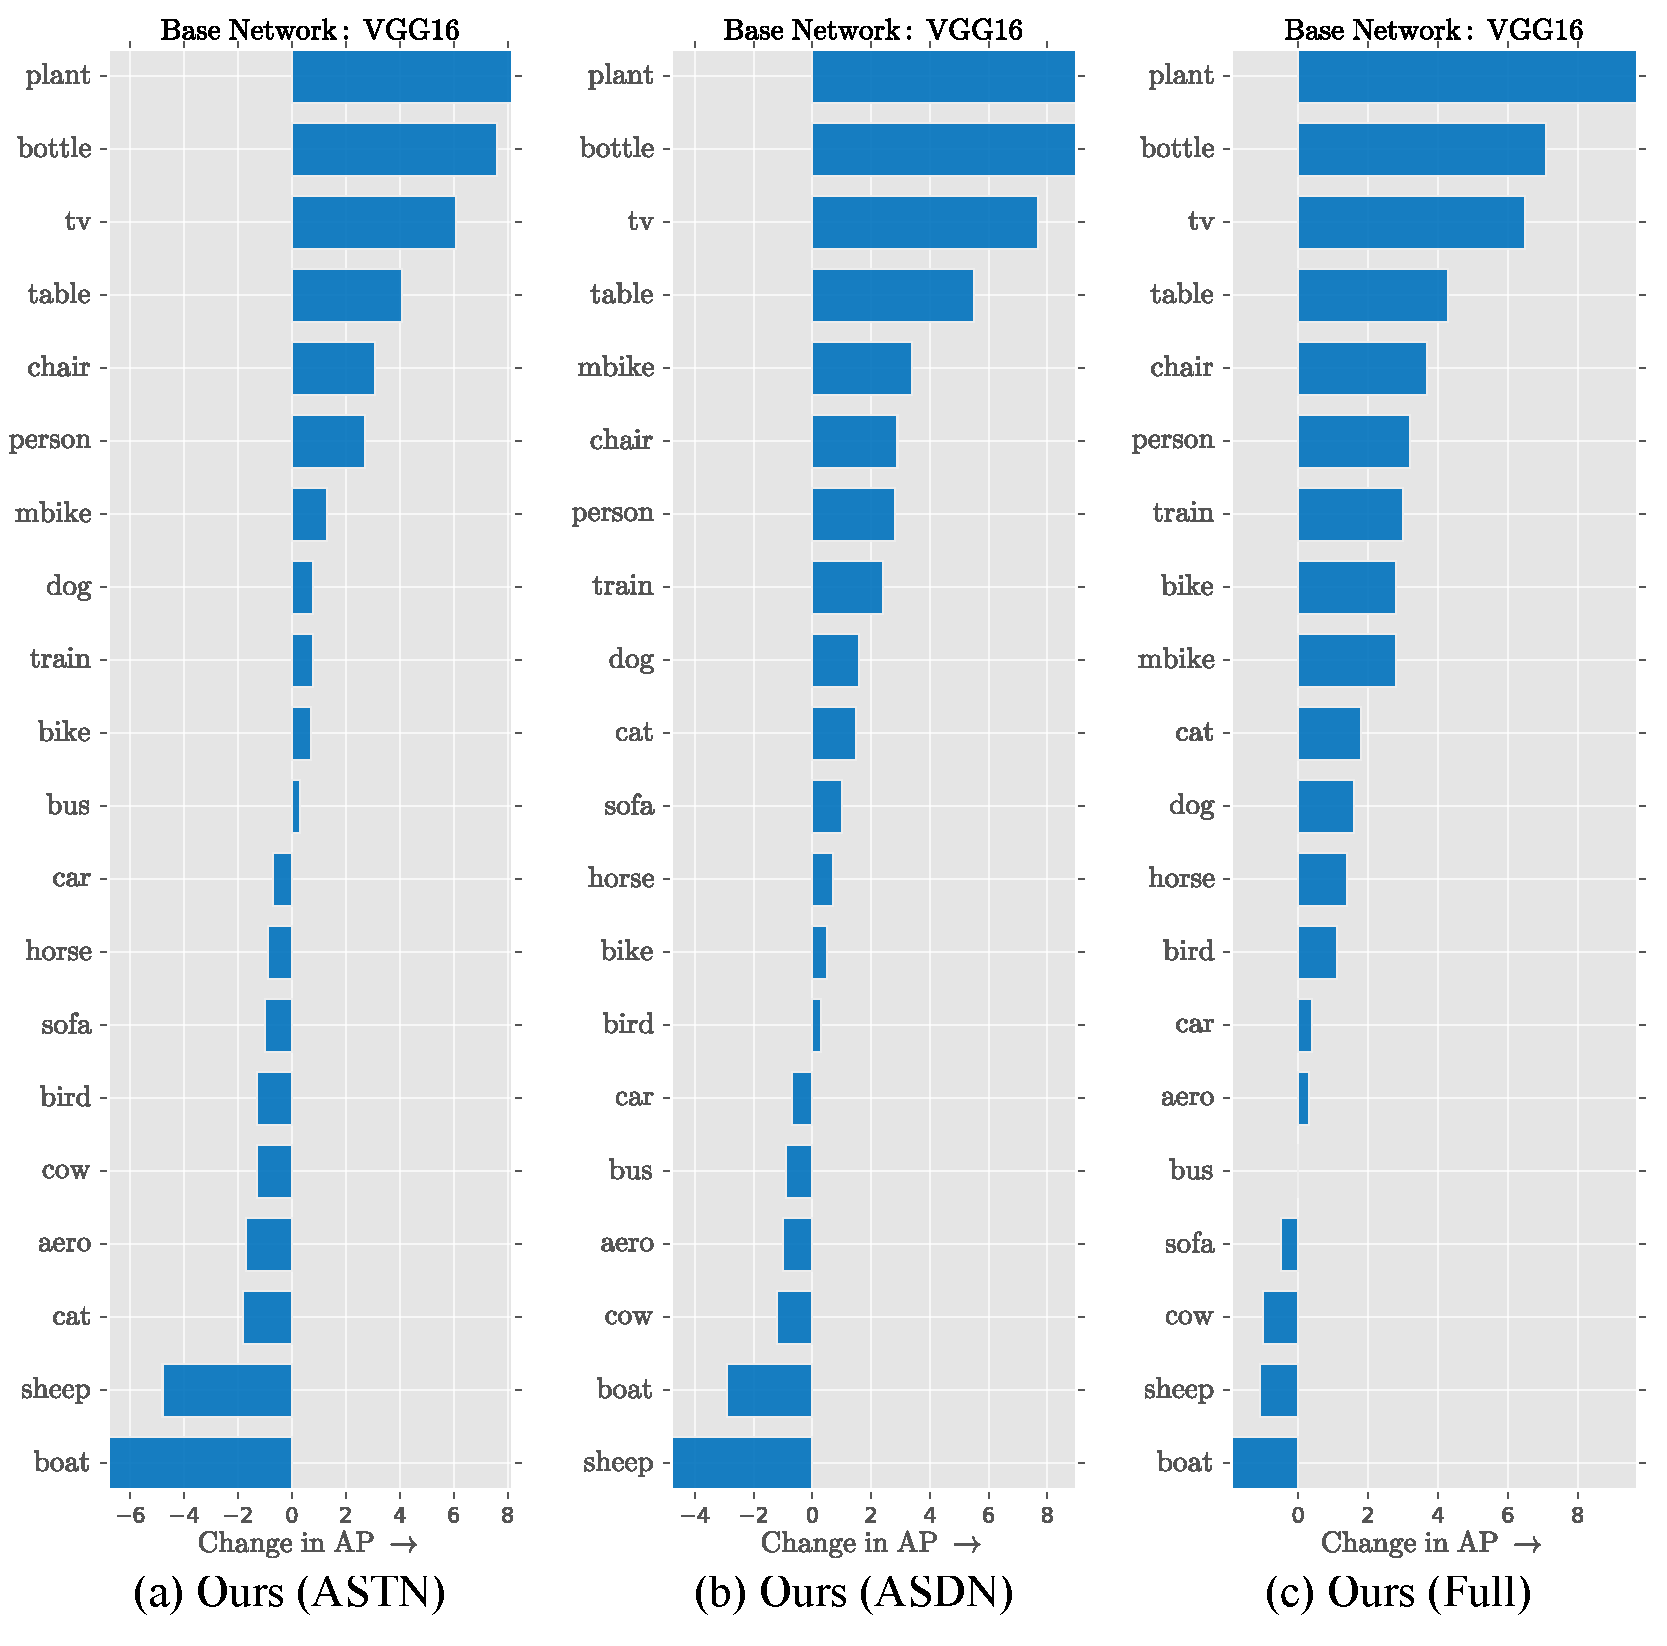
\includegraphics[width=0.95\linewidth]{exp_ap.pdf}
    \vspace{-0.1in}
    \caption{Changes of APs compared to baseline FRCN.}\label{fig:exp_ap}
    \vspace{-0.1in}
\end{figure}
\textbf{ASTN Analysis.} We compared our Adversarial Spatial Transformer Network with random jittering on the object proposals. The augmentations include random changes of scale, aspect ratio and rotation on the proposals during training the Fast-RCNN. With AlexNet, the performance of using random jittering is $57.3\%$ mAP while our ASTN results is $58.1\%$. With VGG16, we have $68.6\%$ for random jittering and $69.9\%$ for the ASTN. For both architectures, the model with ASTN works better than random jittering. 



\vspace{-0.1in}
\subsubsection{Category-based Analysis}
\vspace{-0.05in}
Figure~\ref{fig:exp_ap} shows the graph of how performance of each category changes with the occlusions and deformations. Interestingly the categories that seemed to be helped by both ASTN and ASDN seem to be quire similar. It seems that both {\tt plant} and {\tt bottle} performance improves with adversarial training. However, combining the two transformations together seems to improve performance on some categories which were hurt by using occlusion or deformations alone. Specifically, categories like {\tt car} and {\tt aeroplane} are helped by combining the two adversarial processes.



\subsubsection{Qualitative Results}
\vspace{-0.05in}
Figure~\ref{fig:exp_fp} shows some of the false positives of our approach with the diagnosing code~\cite{hoiem12}. These examples are hand-picked such that they only appeared in the list of false positives for adversarial learning but not the original Fast-RCNN. These results indicate some of the shortcomings of adversarial learning. In some cases, the adversary creates deformations or occlusions which are similar to other object categories and leading to over-generalization. For example, our approach hides the wheels of the bicycle which leads to a wheel chair being classified as a bike. 




\begin{figure}
    \centering
    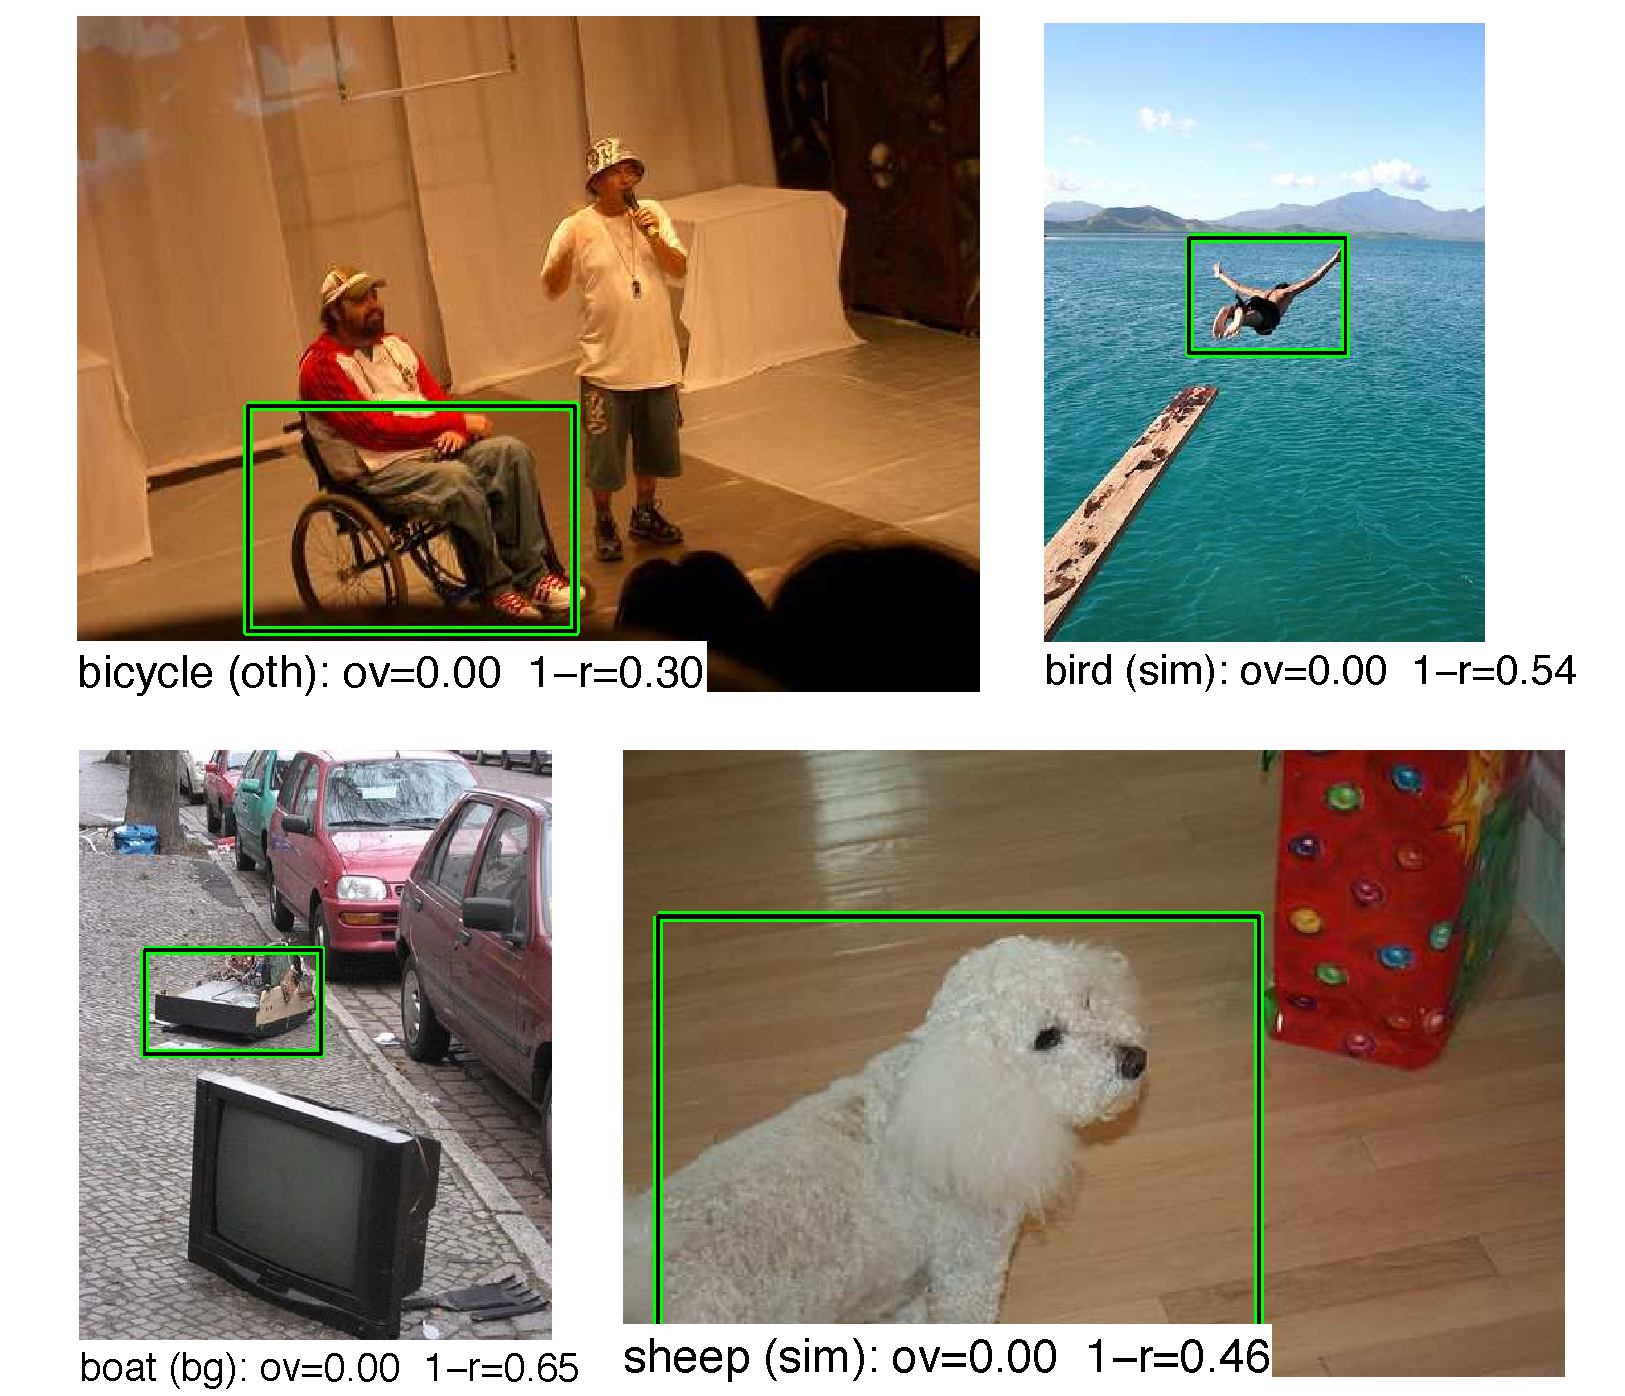
\includegraphics[width=0.95\linewidth]{fp_images.pdf}
    \vspace{-0.1in}
    \caption{Some of the false positives for our approach. These are top false positives for adversarial training but not the original Fast-RCNN.}\label{fig:exp_fp}
    \vspace{-0.15in}
\end{figure}



\subsection{Results on PASCAL VOC 2012 and MS COCO}

We show our results with VGG16 on the PASCAL VOC 2012 dataset in Table~\ref{tab:voc2012}, where our baseline performance is $66.4\%$ .Our full approach with joint learning of ASDN and ASTN gives $2.6\%$ boost to $69.0\%$ mAP. This again shows that the performance improvement using VGG on VOC2012 is significant. We also observe that our method improves performance of all the categories except sofa in VOC 2012. We believe this is probably because of larger diversity in VOC 2012.



We finally report the results in MS COCO dataset. The baseline method with VGG16 architecture is  $42.7\%$ AP$^{50}$ on the VOC metric and $25.7\%$ AP on the standard COCO metric. By applying our method, we achieve $46.2\%$ AP$^{50}$ and $27.1\%$ AP on the VOC and COCO metric respectively. 

\vspace{-0.05in}
\subsection{Comparisons with OHEM}
\vspace{-0.05in}
Our method is also related to the Online Hard Example Mining (OHEM) approach~\cite{shrivastavaOHEM}. Our method allows us to sample data-points which might not exist in the dataset, whereas OHEM is bound by the dataset. However, OHEM has more realistic features since they are extracted from real images. For comparisons, our approach ($71.4\%$) is better than OHEM ($69.9\%$) in VOC2007. However, our result ($69.0\%$) is not as good as OHEM ($69.8\%$) in VOC2012. Since these two approaches are generating or selecting different types of features in training,  we believe they should be complementary. To demonstrate this, we use an ensemble of these two approaches and compare it with separate ensembles of OHEM and Ours alone on VOC 2012. As a result, the ensemble of two methods achieves $71.7\%$ mAP, while the ensemble of two OHEM models ($71.2\%$) or two of our models ($70.2\%$) are not as good, indicating the complementary nature of two approaches. 









